\documentclass{beamer}
%\documentclass[11pt, handout]{beamer}

\usepackage{graphicx}
\usepackage{tikz}
\usepackage{circuitikz}
\usepackage{hyperref}
\usepackage{adjustbox} 
\usetikzlibrary{shapes.geometric, arrows}

%% Alex L's macros 
%% taken and co-opted from a variety of sources
%
%% generic commands
%\newcommand{\NN}{\mathbb{N}}
%\newcommand{\RR}{\mathbb{R}}
%\newcommand{\compindist}{\approx_C}
%
%% definition counter
%\newcounter{defcounter}
%\setcounter{defcounter}{0}
%\newenvironment{definition}{\medskip\noindent\refstepcounter{defcounter}{\bf Definition \thedefcounter}\hspace*{2pt}}{\hspace*{\fill}\nopagebreak[4]$\diamondsuit$\medskip}  
%
%% block quote
%\newenvironment{blockquote}{%
%  \par%
%  \medskip
%  \leftskip=4em\rightskip=2em%
%  \noindent\ignorespaces}{%
%  \par\medskip}
%
%% Author Macros -- colors: red, magenta, blue, orange
%\newcounter{al}
%\newcommand{\al}[1]{\textcolor{blue}{\{AL-\arabic{al}: #1\}}\addtocounter{al}{1}}
%\newcounter{cat}
%\newcommand{\cat}[1]{\textcolor{magenta}{\{CAT-\arabic{cat}: #1\}}\addtocounter{cat}{1}}
%\newcommand{\ignore}[1]{}
%
%% From CompGC paper
%%\renewcommand{\sim}{S}
%%\newcommand{\Input}{\ensuremath{\textsf{Input}}\xspace}
%%\newcommand{\Output}{\ensuremath{\textsf{Output}}\xspace}
%%\newcommand{\Inputs}{\ensuremath{\textsf{Inputs}}\xspace}
%%\newcommand{\Outputs}{\ensuremath{\textsf{Outputs}}\xspace}
%%\newcommand{\Components}{\ensuremath{\textsf{Components}}\xspace}
%
%\newcommand{\Gates}{\text{Gates}}
\newcommand{\C}{\sf {C}}
\newcommand{\GC}{\sf {GC}}
%\newcommand{\AllInputLabels}{\sf {AllInputLabels}}
%\newcommand{\InputLabels}{\sf {InputLabels}}
%\newcommand{\InputWires}{\text{InputWires}}
%\newcommand{\OutputWires}{\text{OutputWires}}
%\newcommand{\Wires}{\text{Wires}}
%\newcommand{\A}{\mathcal{A}}
%\newcommand{\OT}{\textsf{OT}} % or mathsf
\newcommand{\Enc}{\textsf{Enc}} % or mathsf
\newcommand{\Dec}{\textsf{Dec}}
\newcommand{\Gen}{\textsf{Gen}}
\newcommand{\EncInv}{\Enc^{-1}}
\newcommand{\EncDKC}{\textsf{EncDKC}}
\newcommand{\DecDKC}{\textsf{DecDKC}}
\newcommand{\EncDKCInv}{\EncDKC^{-1}}
%\newcommand{\compIndist}{\approx_D}
%\newcommand{\outputrv}{{\sf output}}
%\newcommand{\viewrv}{{\sf view}}
\newcommand{\CompGC}{\textsf{CompGC}\xspace}
%\newcommand{\JustGarble}{\textsf{JustGarble}\xspace}
%\newcommand{\Naive}{\textsf{Naive}\xspace}
%\newcommand{\scmc}{SCMC\xspace} % Single Communication Multiple Connnection


\renewcommand<>{\item}[1]{\only#2{\beameroriginal{\item}{#1}}}
    \mode<presentation> {
        \usetheme{default}
        \usecolortheme{seahorse}
        \setbeamertemplate{footline}[page number] 
        \setbeamertemplate{navigation symbols}{} 
    }

    \title[Short title]{Chaining Garbled Circuits} 
    \author{Alex Ledger} 
    \institute[Reed College]{
        Reed College \\ 
    }
    \date{\today}

    \begin{document}

    \begin{frame}
        \titlepage 
    \end{frame}

    \begin{frame}
        \frametitle{Overview}
        \begin{enumerate}
            \item Secure Computation
            \item Garbled Circuits
            \item Better Garbled Circuits
            \item Chaining Garbled Circuits
            \item Better Chaining of Garbled Circuits
        \end{enumerate}
    \end{frame}

    \begin{frame}
        \frametitle{Goals of this talk}
        \begin{enumerate}
            \item Understand the high level idea of secure computation
                \begin{itemize}
                    \item Maybe you'll run into a situtation where it's useful, and it can help solve an otherwise unsolvable, real world problem.
                \end{itemize}
            \item Understand garbled circuits - the most basic construction
            \item Understand chaining - how we (my thesis) made secure computation faster
            \item We will not be focusing on security (different from most crypto talks)
        \end{enumerate}
        Before we start:
        \begin{enumerate}
            \item Lots of notation: ask me if I brush over something, or you forget what something means.
            \item Lots of moving parts. 
        \end{enumerate}
    \end{frame}

    \begin{frame}
        \frametitle{The Millionaire Problem}
        \begin{itemize}
            \item Alice and Bob want to determine who is wealthier.
            \item They do want to disclose their wealth to each other.
                \begin{itemize}
                    \item Alice has \$$x$, Bob has \$$y$.
                    \item Alice should not learn anything about $y$.
                    \item Bob should not learn anything about $x$.
                \end{itemize}
        \end{itemize}
        \begin{equation}
            f(x,y) = \left\{
                \begin{array}{ll}
                    Alice, & \quad y \leq x; \\
                    Bob, & \quad y > x.
                \end{array}
                \right.
            \end{equation}

            % http://www.alexirpan.com/2016/02/11/secure-computation.html
            \begin{figure}
                \centering
                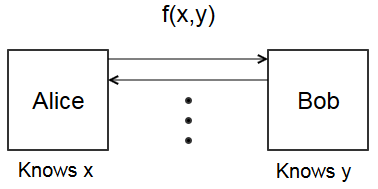
\includegraphics[scale=0.8]{images/setup}
            \end{figure}
        \end{frame}

        \begin{frame}
            \frametitle{Security Properties}
            \begin{itemize}
                \item Privacy of inputs
                    \begin{itemize}
                        \item Alice and Bob do not learn anything about the other's input.
                        \item Except for info that is inferable from $x$ and $f(x,y)$.
                        \item Bob should not learn that $1,000,000 < x \leq 2,000,000$.
                        \item But if $y < x$ and $y = 2,000$, then he learns $x < 2,000$.
                    \end{itemize}
                \item Correctness
                    \begin{itemize}
                        \item Alice and Bob receive $f(x,y)$.
                        \item As opposed to some value near $f(x,y)$.
                        \item Or not receiving a value at all
                    \end{itemize}
                \item Semi-honest
                    \begin{itemize}
                        \item We assume that each party obeys the protocol, but attemps to learn extra information from its  interactions
                    \end{itemize}
            \end{itemize}
        \end{frame}

        \begin{frame}
            \frametitle{Security}
            \begin{figure}
                \centering
                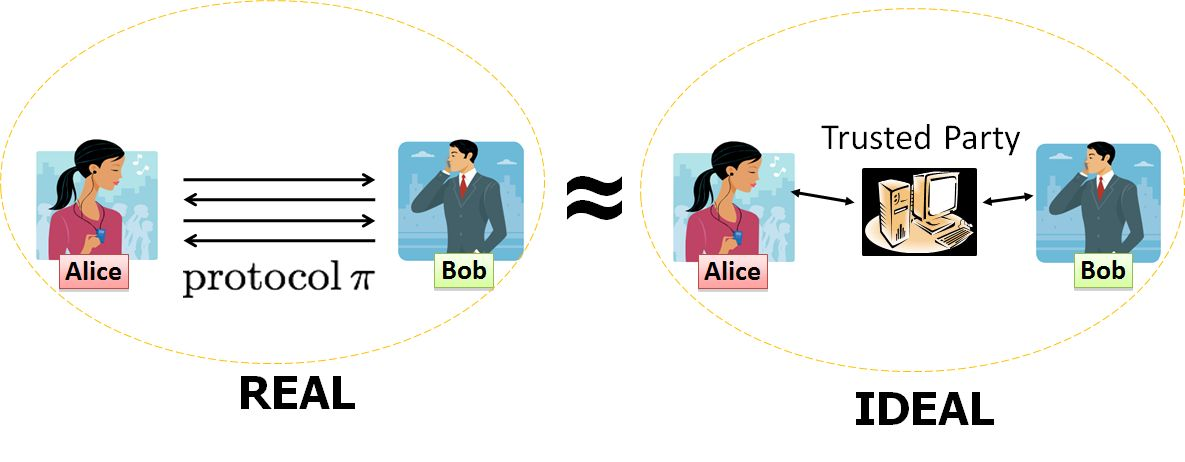
\includegraphics[scale=0.25]{images/security}
            \end{figure}
            A secure computation protocol is secure if Alice and Bob learn the same informatoin in the real world as the ideal world.
        \end{frame}

        \begin{frame}
            \frametitle{Boolean Circuits}
            \begin{itemize}
                \item We encode a function $f$ into a circuit $C$.
                \item Circuit $C$ is made of AND, XOR and NOT gates.
                \item Each gate has two input wires and a single output wire
            \end{itemize}
            \begin{figure}
                \centering
                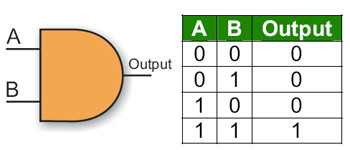
\includegraphics[scale=0.4]{images/and}
                \hfill
                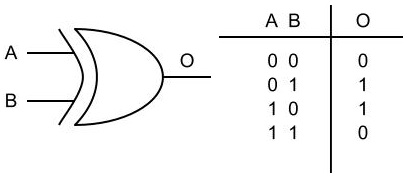
\includegraphics[scale=0.4]{images/xor}
            \end{figure}
        \end{frame}

        \begin{frame}
            \frametitle{Boolean Circuits}
            \begin{itemize}
                \item Any function can be encoded into a circuit.
                \item Here is the less than circuit.
            \end{itemize}
            \begin{figure}
                \centering
                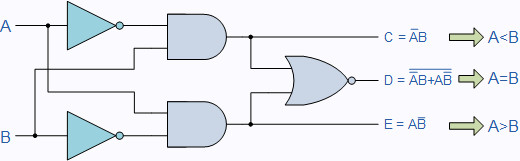
\includegraphics[scale=0.6]{images/less_than}
            \end{figure}
        \end{frame}

        \begin{frame}
            \frametitle{Oblivious Transfer (OT) in brief}
            \begin{itemize}
                \item Alice potentially sends either $m_0$ or $m_1$ to Bob.
                \item Bob receives $m_b$.
                \item Property 1: Alice does not know which message Bob recieved.
                \item Property 2: Bob doesn't anything about $m_{1-b}$.
            \end{itemize}

            \begin{figure}
                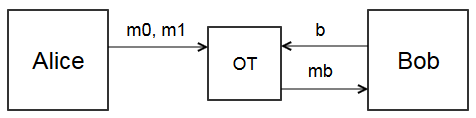
\includegraphics[scale=0.6]{images/ot}
            \end{figure}
        \end{frame}

        \begin{frame}
            \frametitle{Hash Function in brief}
            \begin{itemize}
                \item Hash function $H: \{0,1\}^* \to \{0,1\}^{128}$
                \item For our purposes, $H$ maps any string to a uniform, random 128-bit string.
                \item A.k.a. $H$ is a random oracle.
            \end{itemize}
        \end{frame}

        \begin{frame}
            \frametitle{Roadmap of Garbled Circuits}
            \begin{enumerate}
                    %\item I show how to securely compute a single gate.
                    %    \begin{itemize}
                    %        \item Then we compose many gates to securely compute a circuit.
                    %    \end{itemize}
                \item Suppose Alice and Bob are computing a circuit that is only the AND gate.
                \item Alice \textit{garbles} the AND gate. 
                \item Alice then sends \textit{garbled table} of the gate and some auxiliary information to Bob.
                \item Bob \textit{evaluates} the gate.
            \end{enumerate}

            \begin{figure}
                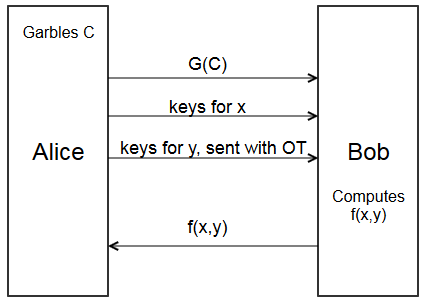
\includegraphics[scale=0.4]{images/high_level}
            \end{figure}
        \end{frame}

        \begin{frame}
            \frametitle{Garbling a gate 1}
            Step 1. Assign \textit{wire labels} to each wire.
            \begin{itemize}
                \item For each wire in the circuit, assign two random labels to each wire
                \item Wire $A$ has wire labels $A_0$ and $A_1$.
                \item We say $A_0$ \textit{semantically represents} $0$, and $A_1$ \textit{semantically represents} $1$.
                \item And $A_0$ and $A_1$ are sampled uniform randomly from $\{0,1\}^n$.
                    \begin{itemize}
                        \item Generally use AES-128 for encryption, so $n = 128$.
                    \end{itemize}
            \end{itemize}

            \begin{figure}
                \label{fig:thefig}
                \centering
                \begin{circuitikz} \draw
                    (0,2) node[and port] (myand1) {}
                    (myand1.in 1) node[left=.8cm](a) {$A_0, A_1$}
                    (myand1.in 2) node[left=.8cm](b) {$B_0, B_1$}
                    (myand1.out) node[right=.25cm](c) {}
                    (myand1.out) node[right=.5cm](d) {$C_0, C_1$}
                    (a) -| (myand1.in 1)
                    (b) -| (myand1.in 2)
                    (myand1.out) -| (c)
                ;\end{circuitikz}
            \end{figure}
        \end{frame}

        \begin{frame}
            \frametitle{Garbling a gate 2}
            Step 2. Construct garbled table.
            \begin{itemize}
                \item Encrypt wire labels for $C$, $C_0$ and $C_1$, using wire labels of $A$ and $B$.
                \item Randomly permute table
            \end{itemize}

            \begin{figure}
                \label{fig:thefig}
                \centering
                \begin{circuitikz} \draw
                    (0,2) node[and port] (myand1) {}
                    (myand1.in 1) node[left=.8cm](a) {$A_0, A_1$}
                    (myand1.in 2) node[left=.8cm](b) {$B_0, B_1$}
                    (myand1.out) node[right=.25cm](c) {}
                    (myand1.out) node[right=.5cm](d) {$C_0, C_1$}
                    (a) -| (myand1.in 1)
                    (b) -| (myand1.in 2)
                    (myand1.out) -| (c)
                ;\end{circuitikz}
            \end{figure}
            \begin{table}
                \centering
                \begin{tabular}{|c|c|c|}
                    \hline
                    $A$ & $B$ & Encryption \\
                    \hline
                    $A_0$ & $B_0$ & $\Enc_{A_0, B_0}(C_0)$ \\
                    $A_1$ & $B_0$ & $\Enc_{A_1, B_0}(C_0)$ \\
                    $A_0$ & $B_1$ & $\Enc_{A_0, B_1}(C_0)$ \\
                    $A_1$ & $B_1$ & $\Enc_{A_1, B_1}(C_1)$ \\                                               
                    \hline
                \end{tabular}
            \end{table}
        \end{frame}

        \begin{frame}
            \frametitle{Garbling a gate 3}
            Step 3. Send garbled table to Bob.
            \begin{table}
                \centering
                \begin{tabular}{|c|}
                    \hline
                    $\Enc_{A_0, B_0}(C_0)$ \\
                    $\Enc_{A_1, B_0}(C_0)$ \\
                    $\Enc_{A_0, B_1}(C_0)$ \\
                    $\Enc_{A_1, B_1}(C_1)$ \\                                               
                    \hline
                \end{tabular}
            \end{table}
        \end{frame}

        \begin{frame}
            \frametitle{Garbling a gate 4}
            Step 4. Send input wire labels to Bob.
            \begin{itemize}
                \item Suppose $x_a, x_b \in \{0,1\}$ are Alice's inputs.
                \item Alice sends Bob $A_{x_a}$ and $B_{x_b}$
                    \begin{itemize}
                        \item The wire labels corresponding to her inputs.
                    \end{itemize}
                \item Bob has:
            \end{itemize}

            \begin{table}
                \begin{tabular}{|c|}
                    \hline
                    Garbled Table \\
                    \hline
                    $\Enc_{A_0, B_0}(C_0)$ \\
                    $\Enc_{A_1, B_0}(C_0)$ \\
                    $\Enc_{A_0, B_1}(C_0)$ \\
                    $\Enc_{A_1, B_1}(C_1)$ \\                                               
                    \hline
                \end{tabular}
                \qquad
                \begin{tabular}{|c|}
                    \hline
                    Input Labels \\
                    \hline
                    $A_*$ \\
                    $B_*$ \\
                    \hline
                \end{tabular}
            \end{table}
        \end{frame}

        \begin{frame}
            \frametitle{Garbling a gate 5}
            Step 5. Bob evaluates the circuit
            \begin{itemize}
                \item Bob has the garbled table, $A_{x_a}$ and $B_{x_b}$.
                \item Bob trial decrypts each row of the garbled table, until an encrytion succeeds.
                \item Bob acquires $C_{a \wedge b}$.
                \item Bob has:
            \end{itemize}
            \begin{table}
                \begin{tabular}{|c|}
                    \hline
                    Garbled Table \\
                    \hline
                    $\Enc_{A_0, B_0}(C_0)$ \\
                    $\Enc_{A_1, B_0}(C_0)$ \\
                    $\Enc_{A_0, B_1}(C_0)$ \\
                    $\Enc_{A_1, B_1}(C_1)$ \\                                               
                    \hline
                \end{tabular}
                \qquad
                \begin{tabular}{|c|}
                    \hline
                    Input Labels \\
                    \hline
                    $A_*$ \\
                    $B_*$ \\
                    \hline
                \end{tabular}
                \qquad
                \begin{tabular}{|c|}
                    \hline
                    Output Label \\
                    \hline 
                    $C_{a \wedge b}$ \\
                    \hline
                \end{tabular}
            \end{table}

        \end{frame}

        \begin{frame}
            \frametitle{Garbling a gate 6}
            Step 6. Bob gets a final answer.
            \begin{itemize}
                \item Alice sends Bob $\Enc_{C_0}(0)$ and $\Enc_{C_1}(1)$.
                \item Bob trial decrypts these with $C_{a \wedge b}$.
                \item One will succeed, and Bob will acquire $c = a \wedge b$.
                \item So Bob knows $c$, but not $a$ and $b$!
            \end{itemize}

            \begin{table}
                \scriptsize
                \begin{tabular}{|c|}
                    \hline
                    Garbled Table \\
                    \hline
                    $\Enc_{A_0, B_0}(C_0)$ \\
                    $\Enc_{A_1, B_0}(C_0)$ \\
                    $\Enc_{A_0, B_1}(C_0)$ \\
                    $\Enc_{A_1, B_1}(C_1)$ \\                                               
                    \hline
                \end{tabular}
                \qquad
                \begin{tabular}{|c|}
                    \hline
                    Input Labels \\
                    \hline
                    $A_a$ \\
                    $B_b$ \\
                    \hline
                \end{tabular}
                \qquad
                \begin{tabular}{|c|}
                    \hline
                    Output Label \\
                    \hline 
                    $C_{a \wedge b}$ \\
                    \hline
                \end{tabular}
                \qquad
                \begin{tabular}{|c|}
                    \hline
                    Output Map \\
                    \hline 
                    $\Enc_{C_0}(0)$ \\
                    $\Enc_{C_1}(1)$ \\
                    \hline
                \end{tabular}
            \end{table}
        \end{frame}

        \begin{frame}
            \frametitle{Security Considerations}
            \begin{itemize}
                \item Think about what Alice acquires:
                    \begin{itemize}
                        \item Well Bob had no input in this case, so ...
                        \item In general, Alice generates objects and sends them to Bob
                        \item So she doesn't have many opportunities to learn about Bob's input.
                    \end{itemize}
                \item Think about what Bob acquires:
                    \begin{enumerate}
                        \item Garbled table
                        \item Input wire labels: $A_a$ and $B_b$
                        \item Encryptions of output: $\Enc_{C_0}(0)$ and $\Enc_{C_1}(1)$
                    \end{enumerate}
                \item Can Bob learn anything about $a$ or $b$?
                    \begin{itemize}
                        \item If he could decrypt another row of the garbled table, then we would learn something.
                            \begin{itemize}
                                \item But he can't, because he doesn't have the keys.
                            \end{itemize}
                        \item Not really, because everything is encrypted.
                    \end{itemize}
            \end{itemize}
        \end{frame}

        \begin{frame}
            \frametitle{Extending a garbled gate into a garbled circuit}
            \begin{itemize}
                \item To operate on a more complex function, the operation is recursed.
                \item The output wires of the first gates are used as inputs to subsequent gates.
                \item Alice only sends output maps for the final gates.
            \end{itemize}
            \begin{figure}
                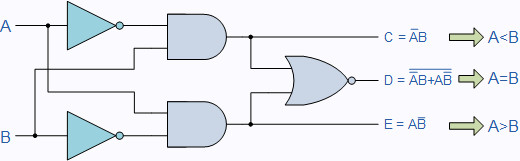
\includegraphics[scale=0.6]{images/less_than}
                %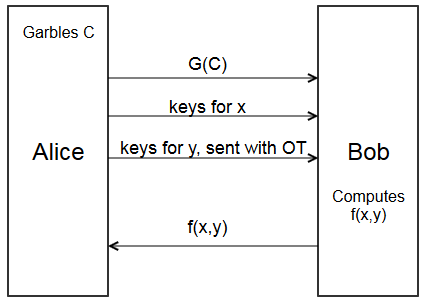
\includegraphics[scale=0.4]{images/high_level}
            \end{figure}
        \end{frame}

        \begin{frame}
            \frametitle{The Garbled Circuit Protocol}
            \begin{figure}
                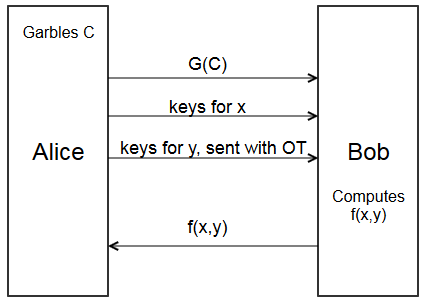
\includegraphics[scale=0.8]{images/high_level}
            \end{figure}
        \end{frame}
        \begin{frame}
            \frametitle{The cost of garbled circuits}
            \begin{itemize}
                \item Alice sends Bob $4$ ciphertexts per gate, since the garbled table has $4$ rows.
                \item This is the bandwidth, or the amount of the communication required.
                \item Based on empirical work, bandwidth is the biggest bottleneck in garbled circuits.
                \item So reducing the size of the garbled table is of utmost priority.
            \end{itemize}
        \end{frame}

        \begin{frame}
            \frametitle{Reducing the size of the garbled table with Free XOR}
            \begin{itemize}
                \item Most improvements to garbled circuits are about choosing wire labels intelligently.
                \item Let $\Delta \gets \{0,1\}^n$ be fixed globally in a circuit.
                \item Let $W_0 \oplus W_1 = \Delta$ for all wires.
                    \begin{itemize}
                        \item aka $W_1 = W_0 \oplus \Delta$.
                        \item We now say that $W_0 = W$.
                    \end{itemize}
                \item Then an XOR gate can be computed by XORing the two input labels.
                \item TODO fix this notation to not use subscripts
                    \begin{align*}
                        A_0 \oplus B_0 & = C_0 \\
                        A_0 \oplus B_1 & = A_0 \oplus (B_0 \oplus \Delta) = (A_0 \oplus B_0) \oplus \Delta = C_1 \\
                        A_1 \oplus B_0 & = (A_0 \oplus \Delta) \oplus B_0 = (A_0 \oplus B_0) \oplus \Delta = C_1 \\
                        A_1 \oplus B_1 & = (A_0 \oplus \Delta) \oplus (B_0 \oplus \Delta) = (A_0 \oplus B_0) = C_0
                    \end{align*}

                \item So XOR gates do not require a garbled table.
                \item They are free
                \item Secure? 
            \end{itemize}
        \end{frame}

        \begin{frame}
            \frametitle{Offline/Online}
            \small
            \begin{itemize}
                \item Imagine two banks use secure computation during their daily operations
                \item At night - the offline phase - they exchange garbled circuits (the garbled tables)
                \item During the day - the online phase - they exchange input wire labels and use the pre-exchanged garbled circuits.
                \item Problems
                    \begin{itemize}
                        \item Functions are decided at night - no room for flexibility
                        \item Input size is fixed at night 
                    \end{itemize}
            \end{itemize}

            \begin{figure}
                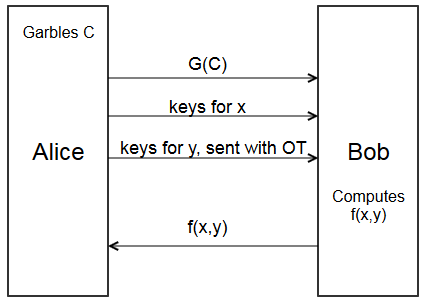
\includegraphics[scale=0.4]{images/high_level}
            \end{figure}
        \end{frame}

        \begin{frame}
            \frametitle{Chaining Garbled Circuits}
            \begin{itemize}
                \item Goal: improve offline/online garbled circuits by adding flexibility
                \item Key observation: many useful functions in the real world are constructed in a modular way
                    \begin{itemize}
                        \item They are composed of standard components
                        \item E.g. addition, subtraction, matrix multiplication
                    \end{itemize}
                \item Idea: chain garbled circuits together
                    \begin{itemize}
                        \item Take the output of one garbled circuit and plug it into another garbled circuit
                    \end{itemize}
            \end{itemize}
            \begin{figure}
                \scalebox{0.75}{
                    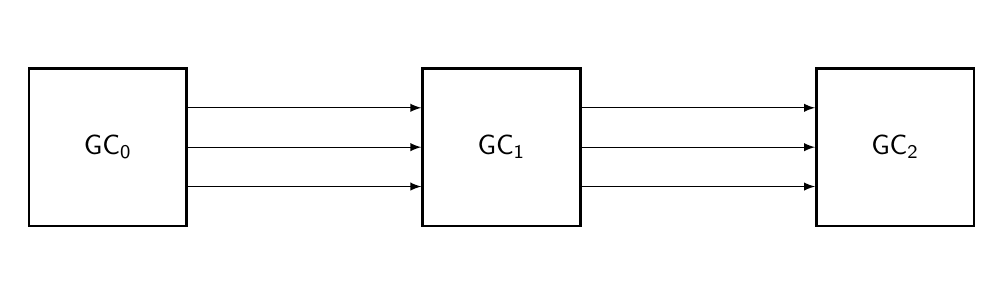
\begin{tikzpicture}
                        [
                            square/.style = {draw, shape=rectangle, minimum height=2cm, minimum width=2cm, node distance=2cm, line width=1pt},
                            empty/.style = {draw, shape=rectangle, minimum height=2cm, minimum width=2cm, node distance=2cm, line width=1pt, draw=white},
                        ]

                        \node[empty] (0a) at (0,0.5)     {};
                        \node[empty] (0b) at (0,-0.5)     {};
                        \node[square] (0c) at (0,0)     {$\GC_0$};

                        \node[empty] (1a) at (5cm,0.5)   {};
                        \node[empty] (1b) at (5cm,-0.5)   {};
                        \node[square] (1c) at (5cm,0)   {$\GC_1$};

                        \node[empty] (2a) at (10cm,0.5)   {};
                        \node[empty] (2b) at (10cm,-0.5)   {};
                        \node[square] (2c) at (10cm,0)   {$\GC_2$};

                        \draw [-latex] (0a.east) -- (1a.west);
                        \draw [-latex] (0b.east) -- (1b.west);
                        \draw [-latex] (0c.east) -- (1c.west);

                        \draw [-latex] (1a.east) -- (2a.west);
                        \draw [-latex] (1b.east) -- (2b.west);
                        \draw [-latex] (1c.east) -- (2c.west);

                    \end{tikzpicture}
                }
            \end{figure}

        \end{frame}

        \begin{frame}
            \frametitle{How to chain garbled circuits}
            \begin{itemize}
                \item Suppose that we are chaining a garbled circuit with output wire $A$ to garbled circuit with input wire $X$.
                \item We want $A \to B$ and $X \oplus \Delta \to X \oplus \Delta$.
                \item Straightforward:
                    \begin{itemize}
                        \item Alice sends Bob {\color{blue}$W_{AB}$}$ = A \oplus B$
                        \item Bob sets $B_* \gets A_* \oplus$ {\color{blue}$W_{AB}$}
                    \end{itemize}

                    \begin{figure}
                        \scalebox{0.75}{
                            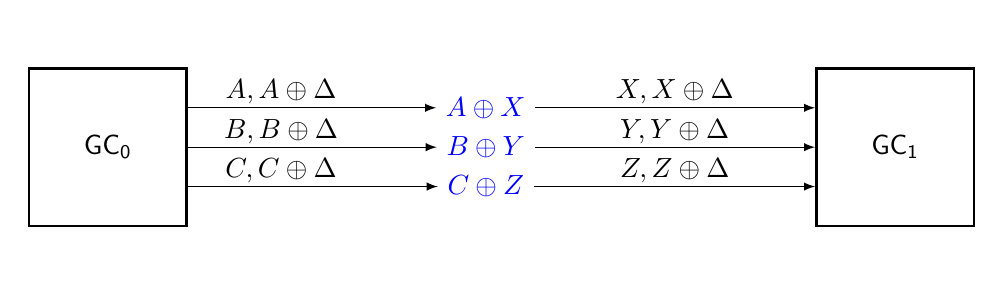
\begin{tikzpicture}
                                [
                                    square/.style = {draw, shape=rectangle, minimum height=2cm, minimum width=2cm, node distance=2cm, line width=1pt},
                                    empty/.style = {draw, shape=rectangle, minimum height=2cm, minimum width=2cm, node distance=2cm, line width=1pt, draw=white},
                                ]

                                \node[empty] (0a) at (0,0.5)     {};
                                \node[empty] (0b) at (0,-0.5)     {};
                                \node[square] (0c) at (0,0)     {$\GC_0$};

                                \node[color=blue] (mida) at (4.8cm,0.5)   {$A \oplus X$};
                                \node[color=blue] (midb) at (4.8cm,-0.5)  {$C \oplus Z$}; 
                                \node[color=blue] (midc) at (4.8cm,0)     {$B \oplus Y$};

                                \node[empty] (1a) at (10cm,0.5)   {};
                                \node[empty] (1b) at (10cm,-0.5)   {};
                                \node[square] (1c) at (10cm,0)   {$\GC_1$};

                                \node (x0) at (2.2cm,0.7) {$A, A \oplus \Delta$};
                                \node (y0) at (2.2cm,-0.3) {$C, C \oplus \Delta$};
                                \node (z0) at (2.2cm,0.2) {$B, B \oplus \Delta$};

                                \node (x1) at (7.2cm,0.7) {$X, X \oplus \Delta$};
                                \node (y1) at (7.2cm,-0.3) {$Z, Z \oplus \Delta$};
                                \node (z1) at (7.2cm,0.2) {$Y, Y \oplus \Delta$};

                                \draw [-latex] (0a.east) -- (mida.west);
                                \draw [-latex] (0b.east) -- (midb.west);
                                \draw [-latex] (0c.east) -- (midc.west);

                                \draw [-latex] (mida.east) -- (1a.west);
                                \draw [-latex] (midb.east) -- (1b.west);
                                \draw [-latex] (midc.east) -- (1c.west);
                            \end{tikzpicture}
                        }
                    \end{figure}
                    \pause
                \item Is this secure? What does Bob learn?
                    \begin{itemize}
                        \item Not really anything.
                    \end{itemize}
            \end{itemize}
        \end{frame}

        \begin{frame}
            \frametitle{Efficienty of chaining garbled circuits}
            \begin{itemize}
                \item In online phase, chaining requires communicating a ciphertext per chain
                \item This can be a lot of communication
                    \begin{itemize}
                        \item Suppose $100$ by $100$ matrix with entries of max value $2^8$
                        \item Then requires $256,000$ ciphertexts
                        \item That's 4 megabytes!
                    \end{itemize}
                \item We can reduce this chaining to a single ciphertext
            \end{itemize}
        \end{frame}

        \begin{frame}
            \frametitle{Single Communication Multiple Connections SCMC}
            \begin{itemize}
                \item Problem: number of ciphertexts communicated scales linearly with the number of chains
                \item Key observation: the chaining is predictable, consecutive wires are chained to consecutive wires
                \item Solution: give consecutive wire labels a predictable pattern
            \end{itemize}

            \begin{figure}
                \scalebox{0.75}{
                    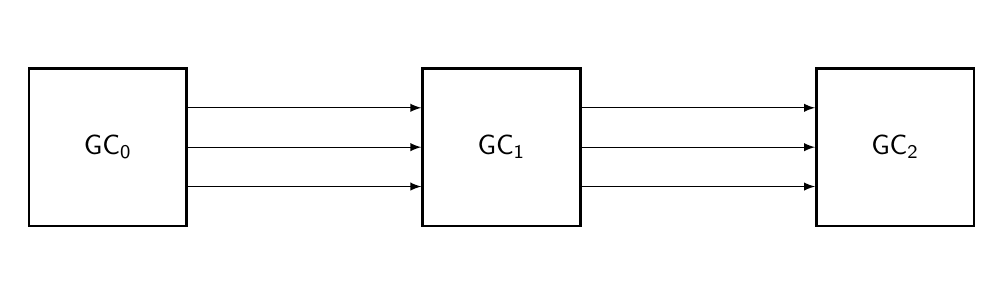
\begin{tikzpicture}
                        [
                            square/.style = {draw, shape=rectangle, minimum height=2cm, minimum width=2cm, node distance=2cm, line width=1pt},
                            empty/.style = {draw, shape=rectangle, minimum height=2cm, minimum width=2cm, node distance=2cm, line width=1pt, draw=white},
                        ]

                        \node[empty] (0a) at (0,0.5)     {};
                        \node[empty] (0b) at (0,-0.5)     {};
                        \node[square] (0c) at (0,0)     {$\GC_0$};

                        \node[empty] (1a) at (5cm,0.5)   {};
                        \node[empty] (1b) at (5cm,-0.5)   {};
                        \node[square] (1c) at (5cm,0)   {$\GC_1$};

                        \node[empty] (2a) at (10cm,0.5)   {};
                        \node[empty] (2b) at (10cm,-0.5)   {};
                        \node[square] (2c) at (10cm,0)   {$\GC_2$};

                        \draw [-latex] (0a.east) -- (1a.west);
                        \draw [-latex] (0b.east) -- (1b.west);
                        \draw [-latex] (0c.east) -- (1c.west);

                        \draw [-latex] (1a.east) -- (2a.west);
                        \draw [-latex] (1b.east) -- (2b.west);
                        \draw [-latex] (1c.east) -- (2c.west);

                    \end{tikzpicture}
                }
            \end{figure}


        \end{frame}

        \begin{frame}
            \frametitle{Single Communcation Multiple Connections SCMC}
            % http://tex.stackexchange.com/questions/201071/how-do-i-make-tikz-circular-arrowheads-concentric-to-the-point-they-connect
            \begin{itemize}
                \item Set $i$th input wire label of circuit to $A \oplus H(i)$.
                \item Set $j$th output wire label of circuit to $X \oplus H(j)$.
                    \begin{itemize}
                        \item Technically, we the labels to $A \oplus H (T \oplus (i || b))$
                        \item Where $H$ is a hash function or a random oracle
                    \end{itemize}
            \end{itemize}

            \begin{figure}
                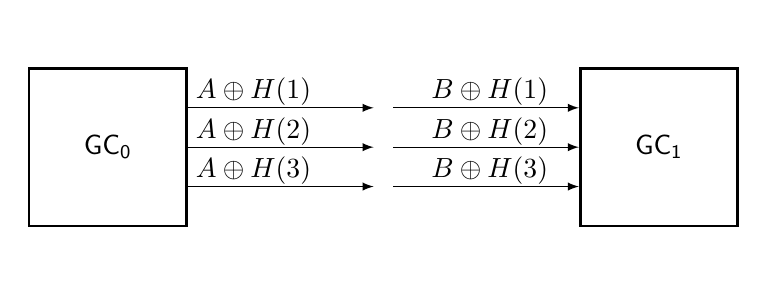
\begin{tikzpicture}
                    [
                        square/.style = {draw, shape=rectangle, minimum height=2cm, minimum width=2cm, node distance=2cm, line width=1pt},
                        empty/.style = {draw, shape=rectangle, minimum height=2cm, minimum width=2cm, node distance=2cm, line width=1pt, draw=white},
                    ]

                    \node[empty] (0a) at (0,0.5)     {};
                    \node[empty] (0b) at (0,-0.5)     {};
                    \node[square] (0c) at (0,0)     {$\GC_0$};

                    \node (mida) at (3.5cm,0.5)     {};
                    \node (midb) at (3.5cm,-0.5)     {};
                    \node (midc) at (3.5cm,0)     {};

                    \node[empty] (1a) at (7cm,0.5)   {};
                    \node[empty] (1b) at (7cm,-0.5)   {};
                    \node[square] (1c) at (7cm,0)   {$\GC_1$};

                    \node (x0) at (1.85cm,0.7) {$A \oplus H(1)$};
                    \node (y0) at (1.85cm,-0.3) {$A \oplus H(3)$};
                    \node (z0) at (1.85cm,0.2) {$A \oplus H(2)$};

                    \node (x1) at (4.85cm,0.7) {$B \oplus H(1)$};
                    \node (y1) at (4.85cm,-0.3) {$B \oplus H(3)$};
                    \node (z1) at (4.85cm,0.2) {$B \oplus H(2)$};

                    \draw [-latex] (0a.east) -- (mida);
                    \draw [-latex] (0b.east) -- (midb);
                    \draw [-latex] (0c.east) -- (midc);

                    \draw [-latex] (mida) -- (1a.west);
                    \draw [-latex] (midb) -- (1b.west);
                    \draw [-latex] (midc) -- (1c.west);
                \end{tikzpicture}
            \end{figure}
        \end{frame}

        \begin{frame}
            \frametitle{My thesis work}
            \begin{itemize}
                \item I implemented naive chaining and SCMC in a system called \CompGC
                \item Written in C
                \item I started with JustGarble
                    \begin{itemize}
                        \item Garbled circuits and evaluated them
                        \item The state of the art in speed
                        \item A colleague added some features to make it faster.
                    \end{itemize}
            \end{itemize}
        \end{frame}
        \end{document} 






